% Options for packages loaded elsewhere
\PassOptionsToPackage{unicode}{hyperref}
\PassOptionsToPackage{hyphens}{url}
%
\documentclass[
]{article}
\title{Exploratory Data Analysis}
\author{Jyotsna Verma}
\date{12/11/2021}

\usepackage{amsmath,amssymb}
\usepackage{lmodern}
\usepackage{iftex}
\ifPDFTeX
  \usepackage[T1]{fontenc}
  \usepackage[utf8]{inputenc}
  \usepackage{textcomp} % provide euro and other symbols
\else % if luatex or xetex
  \usepackage{unicode-math}
  \defaultfontfeatures{Scale=MatchLowercase}
  \defaultfontfeatures[\rmfamily]{Ligatures=TeX,Scale=1}
\fi
% Use upquote if available, for straight quotes in verbatim environments
\IfFileExists{upquote.sty}{\usepackage{upquote}}{}
\IfFileExists{microtype.sty}{% use microtype if available
  \usepackage[]{microtype}
  \UseMicrotypeSet[protrusion]{basicmath} % disable protrusion for tt fonts
}{}
\makeatletter
\@ifundefined{KOMAClassName}{% if non-KOMA class
  \IfFileExists{parskip.sty}{%
    \usepackage{parskip}
  }{% else
    \setlength{\parindent}{0pt}
    \setlength{\parskip}{6pt plus 2pt minus 1pt}}
}{% if KOMA class
  \KOMAoptions{parskip=half}}
\makeatother
\usepackage{xcolor}
\IfFileExists{xurl.sty}{\usepackage{xurl}}{} % add URL line breaks if available
\IfFileExists{bookmark.sty}{\usepackage{bookmark}}{\usepackage{hyperref}}
\hypersetup{
  pdftitle={Exploratory Data Analysis},
  pdfauthor={Jyotsna Verma},
  hidelinks,
  pdfcreator={LaTeX via pandoc}}
\urlstyle{same} % disable monospaced font for URLs
\usepackage[margin=1in]{geometry}
\usepackage{graphicx}
\makeatletter
\def\maxwidth{\ifdim\Gin@nat@width>\linewidth\linewidth\else\Gin@nat@width\fi}
\def\maxheight{\ifdim\Gin@nat@height>\textheight\textheight\else\Gin@nat@height\fi}
\makeatother
% Scale images if necessary, so that they will not overflow the page
% margins by default, and it is still possible to overwrite the defaults
% using explicit options in \includegraphics[width, height, ...]{}
\setkeys{Gin}{width=\maxwidth,height=\maxheight,keepaspectratio}
% Set default figure placement to htbp
\makeatletter
\def\fps@figure{htbp}
\makeatother
\setlength{\emergencystretch}{3em} % prevent overfull lines
\providecommand{\tightlist}{%
  \setlength{\itemsep}{0pt}\setlength{\parskip}{0pt}}
\setcounter{secnumdepth}{-\maxdimen} % remove section numbering
\ifLuaTeX
  \usepackage{selnolig}  % disable illegal ligatures
\fi

\begin{document}
\maketitle

\textbf{Introduction - }

Massive Open Online Courses (MOOCs) are free online courses available
for anyone to enroll. MOOCs have dramatically changed the way the world
learns by providing an affordable and flexible way to learn new skills,
help in career advancements etc. There is a very vast amount of data
produced by e-learning systems and the measurement, collection, analysis
and reporting of this data about learners can help a business a lot in
optimizing learning experience and the environment in which it occurs

This project is about extracting insights from learners' data provided
by an online course provider Future Learn for a cyber security course.

\textbf{Business Understanding }

In this project we are analyzing, exploring, transforming and gathering
the past information from the data and using it to improve our course
for future batches based on past learning and experience.

\textbf{Data Understanding:}

We have data of 7 batches which was run in a span of 2 years from 2016
to 2018.

We have 7 sets of static as well as fluid data for each batch which
gives us the details about the student records, and the students'
interaction with the virtual course. There different datasets for all
the seven batches are:

\begin{enumerate}
\def\labelenumi{\arabic{enumi})}
\item
  Archetype survey response -- it gives the details about the learners
  and their archetype, that is how they intend to use this course for.
\item
  Enrolments -- this gives the students' details and information, and
  their enrolment details and the full participation in the course
  (course completion, that is purchased the upgraded course
  certificates).
\item
  Leaving survey response -- this data set gives us an idea of the
  learners who left the course when (the timestamp as well as the last
  step at which they left the course) and the reason of leaving.
\item
  Question response -- this dataset gives us the details of the
  assessment in the course.
\item
  Step activity -- this dataset gives us the details of the
  steps(topics) and if the learners visited and completed that topic (or
  step)
\item
  Team members -- this dataset gives us the knowledge of the role of the
  user in the course and their role in their team.
\item
  Video stats -- this dataset gives us the details of the video modules
  in the course. It gives us the description of the video duration of
  the topics, the total no of views, number of people who downloaded the
  video and other details how people accessed these video modules. It
  also gives us the information about the percentage length of each
  video viewed. It provides us with the information of the devices which
  were used to access the videos and the information about the views
  from all the continents.
\item
  Weekly sentiment survey -- this dataset gives the details about the
  feedback from the learners for the weekly modules.
\end{enumerate}

We have similar types of files for all the seven batches. The number
1,2,3\ldots and so on in the file names represent the batch number.

The data for enrolments, question response and step activity are
provided for all the seven batches. The archetype survey response data
and the data set containing the details of the video stats is not
provided for batch number 1 and 2, but is available for all the other
batches. The leaving survey response data is provided only for the
batches 4,5,6 \& 7. The data for team members is provided for all the
batches except for the first batch. The weekly sentiment survey dataset
is only available for the batches 5, 6 and 7 where batch 5 contains the
response from just one learner.

After examining the basic properties, summary and the details of the
data we discovered that a lot of the entries in the data set are
``Unknown'' or have missing values.

So, we have done our analysis and visualizations on the data that is
provided to us excluding the unknown values (that constitutes a
significant amount of data). So, this analysis may or may not give exact
results and the insights.

\textbf{Business Objective }

\begin{itemize}
\tightlist
\item
  Our first objective for this project is targeting the serious
  learners, and audience and increasing the retention of the student for
  the course.
\end{itemize}

\textbf{Data Description }

Here for this analysis, we are using the enrolments dataset and the
archetype dataset from all the seven batches to see what kind of
learners are interested in the course and how well these insights can be
used to achieve our goal. We have used the leaving response survey data
set from all the seven batches to analyze what is the most common reason
for people leaving the course.

We will also be analyzing the total view, transcript views, captions and
HD viewing.

\textbf{Data Preparation: }

The data from the same type of dataset from all the seven batches are
merged to get an overview of the kind of learners and for other analysis
of the course. Here we have merged the enrolments dataset of all the 7
batches to get an overall view of the trend and the characteristics of
the learners.

The enrolment dataset and the archetype dataset from all the batches are
also merged to get an idea about the learners that how they intend to
use this course for.

Here in these datasets, we can see that the data is not very consistent
and we have a lot of missing values and some of the entries as
``Unknown'', so we have done the analysis leaving the unknown values. In

Again, in the enrolment's dataset, we have country columns and the
detected country columns, there are a lot of missing values in the
country column, so we have carried out our analysis on the basis of
detected country column. Moreover in the same dataset we have roles
defined as Learners and Organisational admin. We have done our analysis
for all the learners (the organisation admin entries were excluded when
we excluded the unknown values from different variables)

For analyzing the views from video stats dataset,We are using the data
from merged video\_stats. We summarized the columns containing total
views, total caption views, total transcript views and viewed\_HD. Then
we used melt function to organize the data. (Here all the data from
those 4 columns were stacked into a single column). Then this data frame
was used for our analysis.

\textbf{Evaluation/ Data Analysis:}

Here we are checking the trend of the learners who enroll in the course
and the ones who fully participated in the course.

Fig 1. this gives the trend of all the learners from all the 7 batches
who enrolled for the course as well as who completed the course.

\begin{figure}
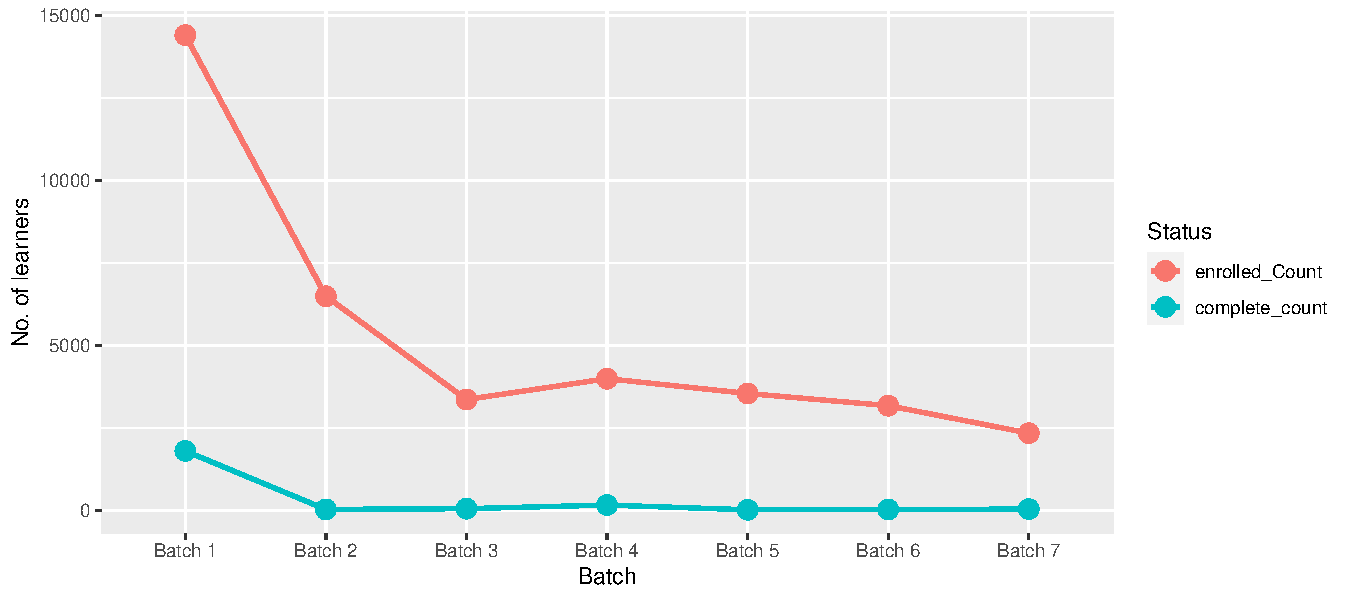
\includegraphics[width=1\linewidth]{CSC8631-Reports_files/figure-latex/unnamed-chunk-1-1} \caption{Trend of learners who enrolled and who fully participated across all batches}\label{fig:unnamed-chunk-1}
\end{figure}

Here we can see highest number of learners enrolling in the first batch
and then the no. Of participants decreases significantly. We can see
that there is an increase in the number of participants for the 4th
batch but after that it has shown a decreasing trend. We observe that
there is significant difference in the number of learners who have
enrolled and the ones who have completed the course. This can be
analyzed further with leaving survey response dataset which contains the
reason for participants leaving the course.

Fig 2. gives a visual analysis of the leaving response by the learners.

\begin{figure}
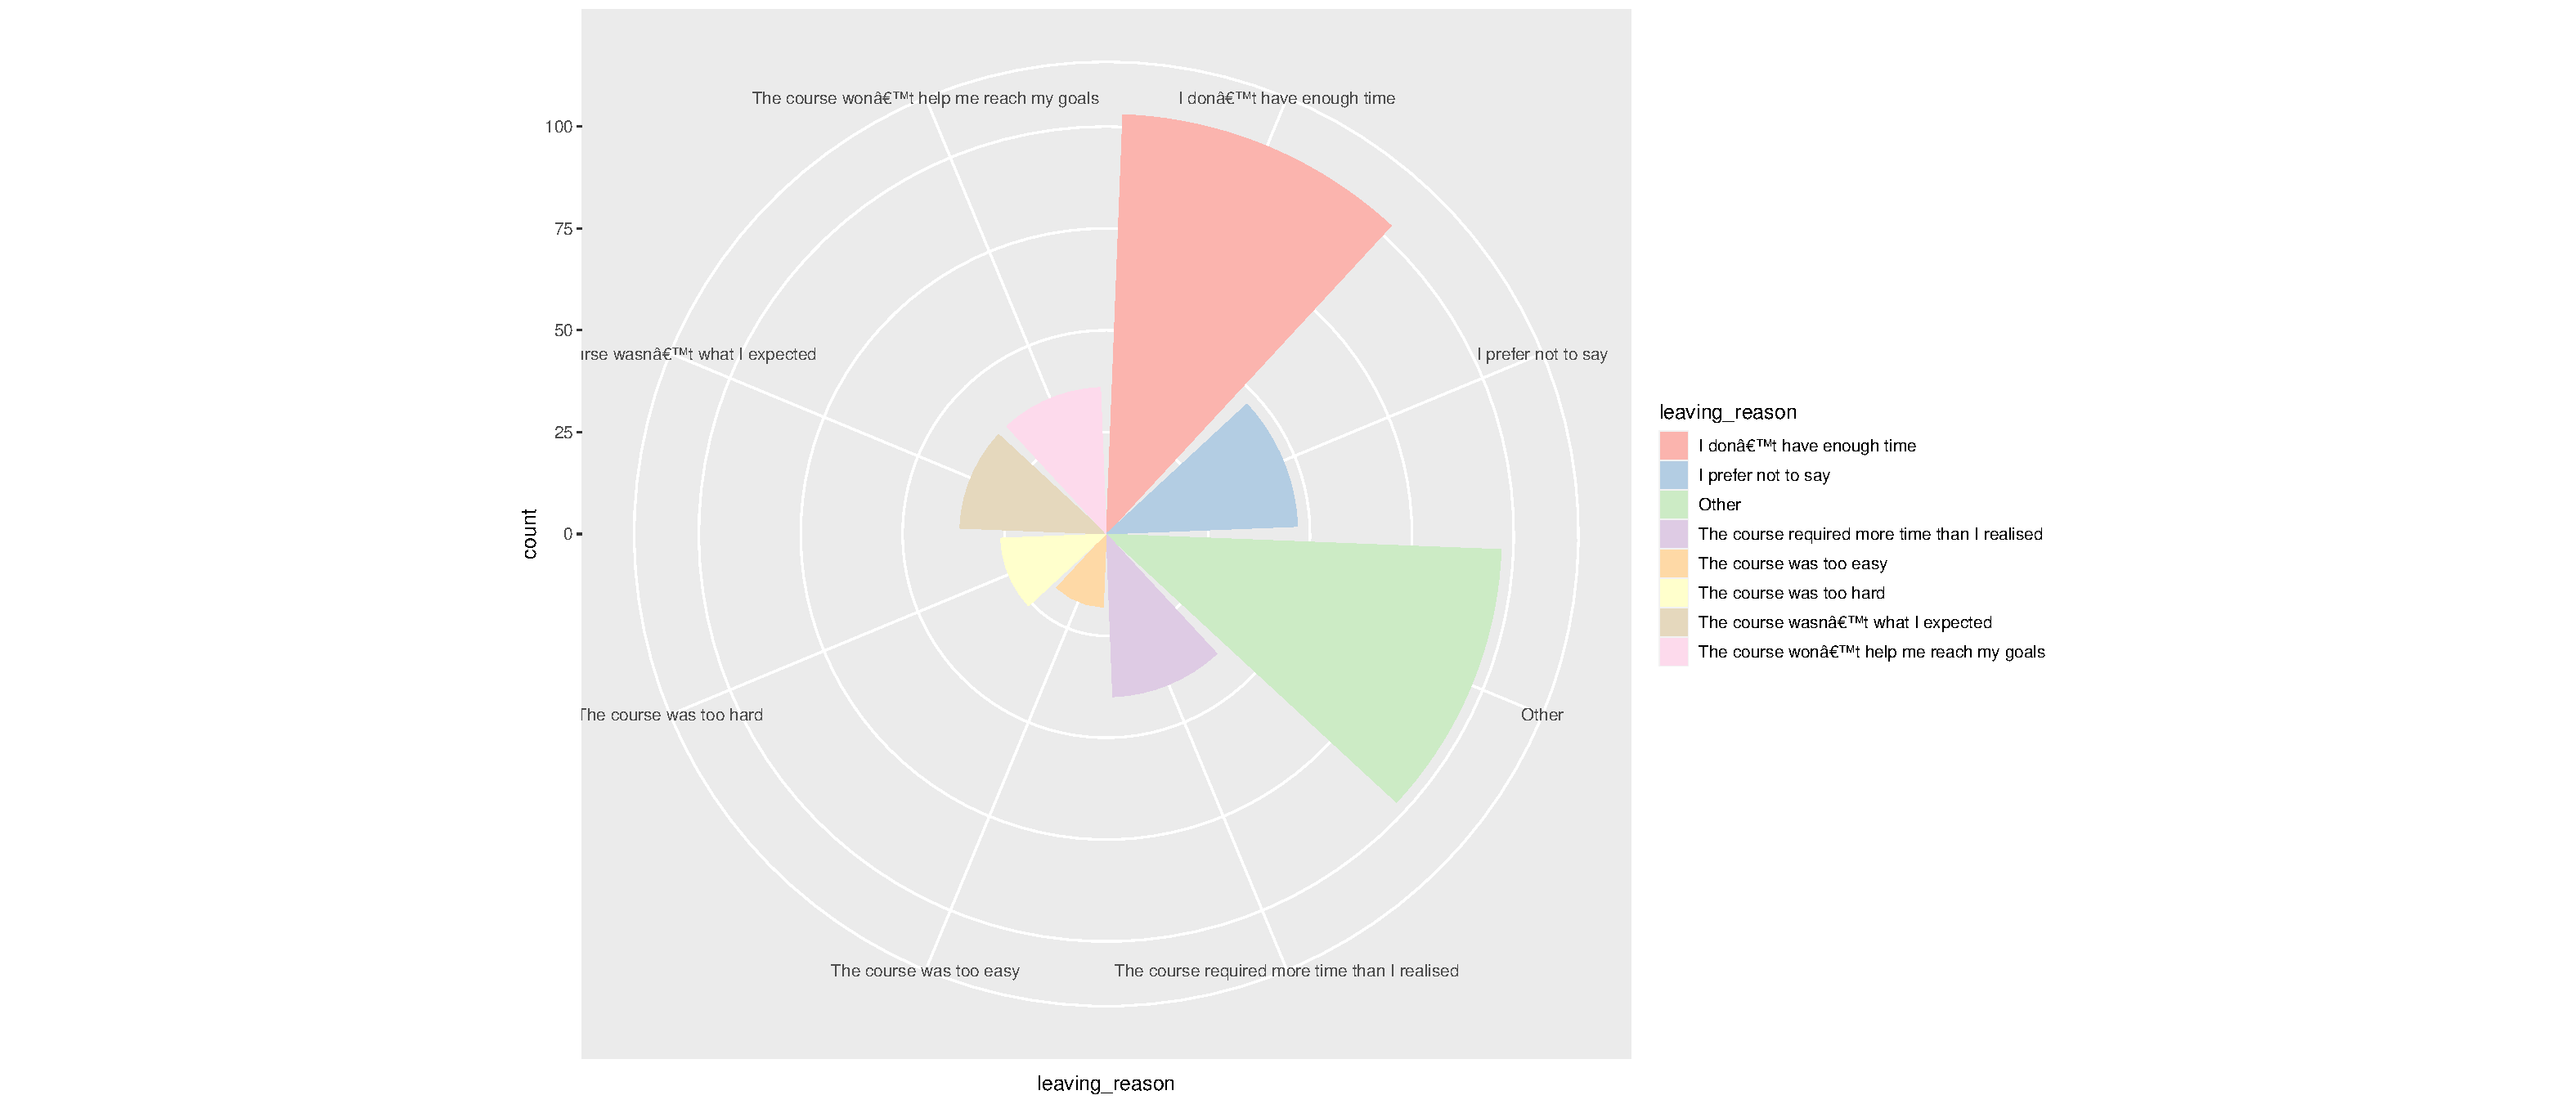
\includegraphics[width=1\linewidth]{CSC8631-Reports_files/figure-latex/unnamed-chunk-2-1} \caption{Leaving response of the learners}\label{fig:unnamed-chunk-2}
\end{figure}

This shows that most of the learners who left the course have mentioned
the reason of not having enough time. The reason about course requiring
more time than expected is also chosen by a lot of learners, which
depicts the same reason of learners struggling with time. Here we can
further check what kind of learneres are involved and how can this issue
be resolved.

Now, here fig 3 shows the Combined overview of learners who enrolled for
the course and the ones who fully participated in the program (purchased
the upgraded course certificates). For this we will be using our merged
enrolments dataset from all the seven batches.

\begin{figure}
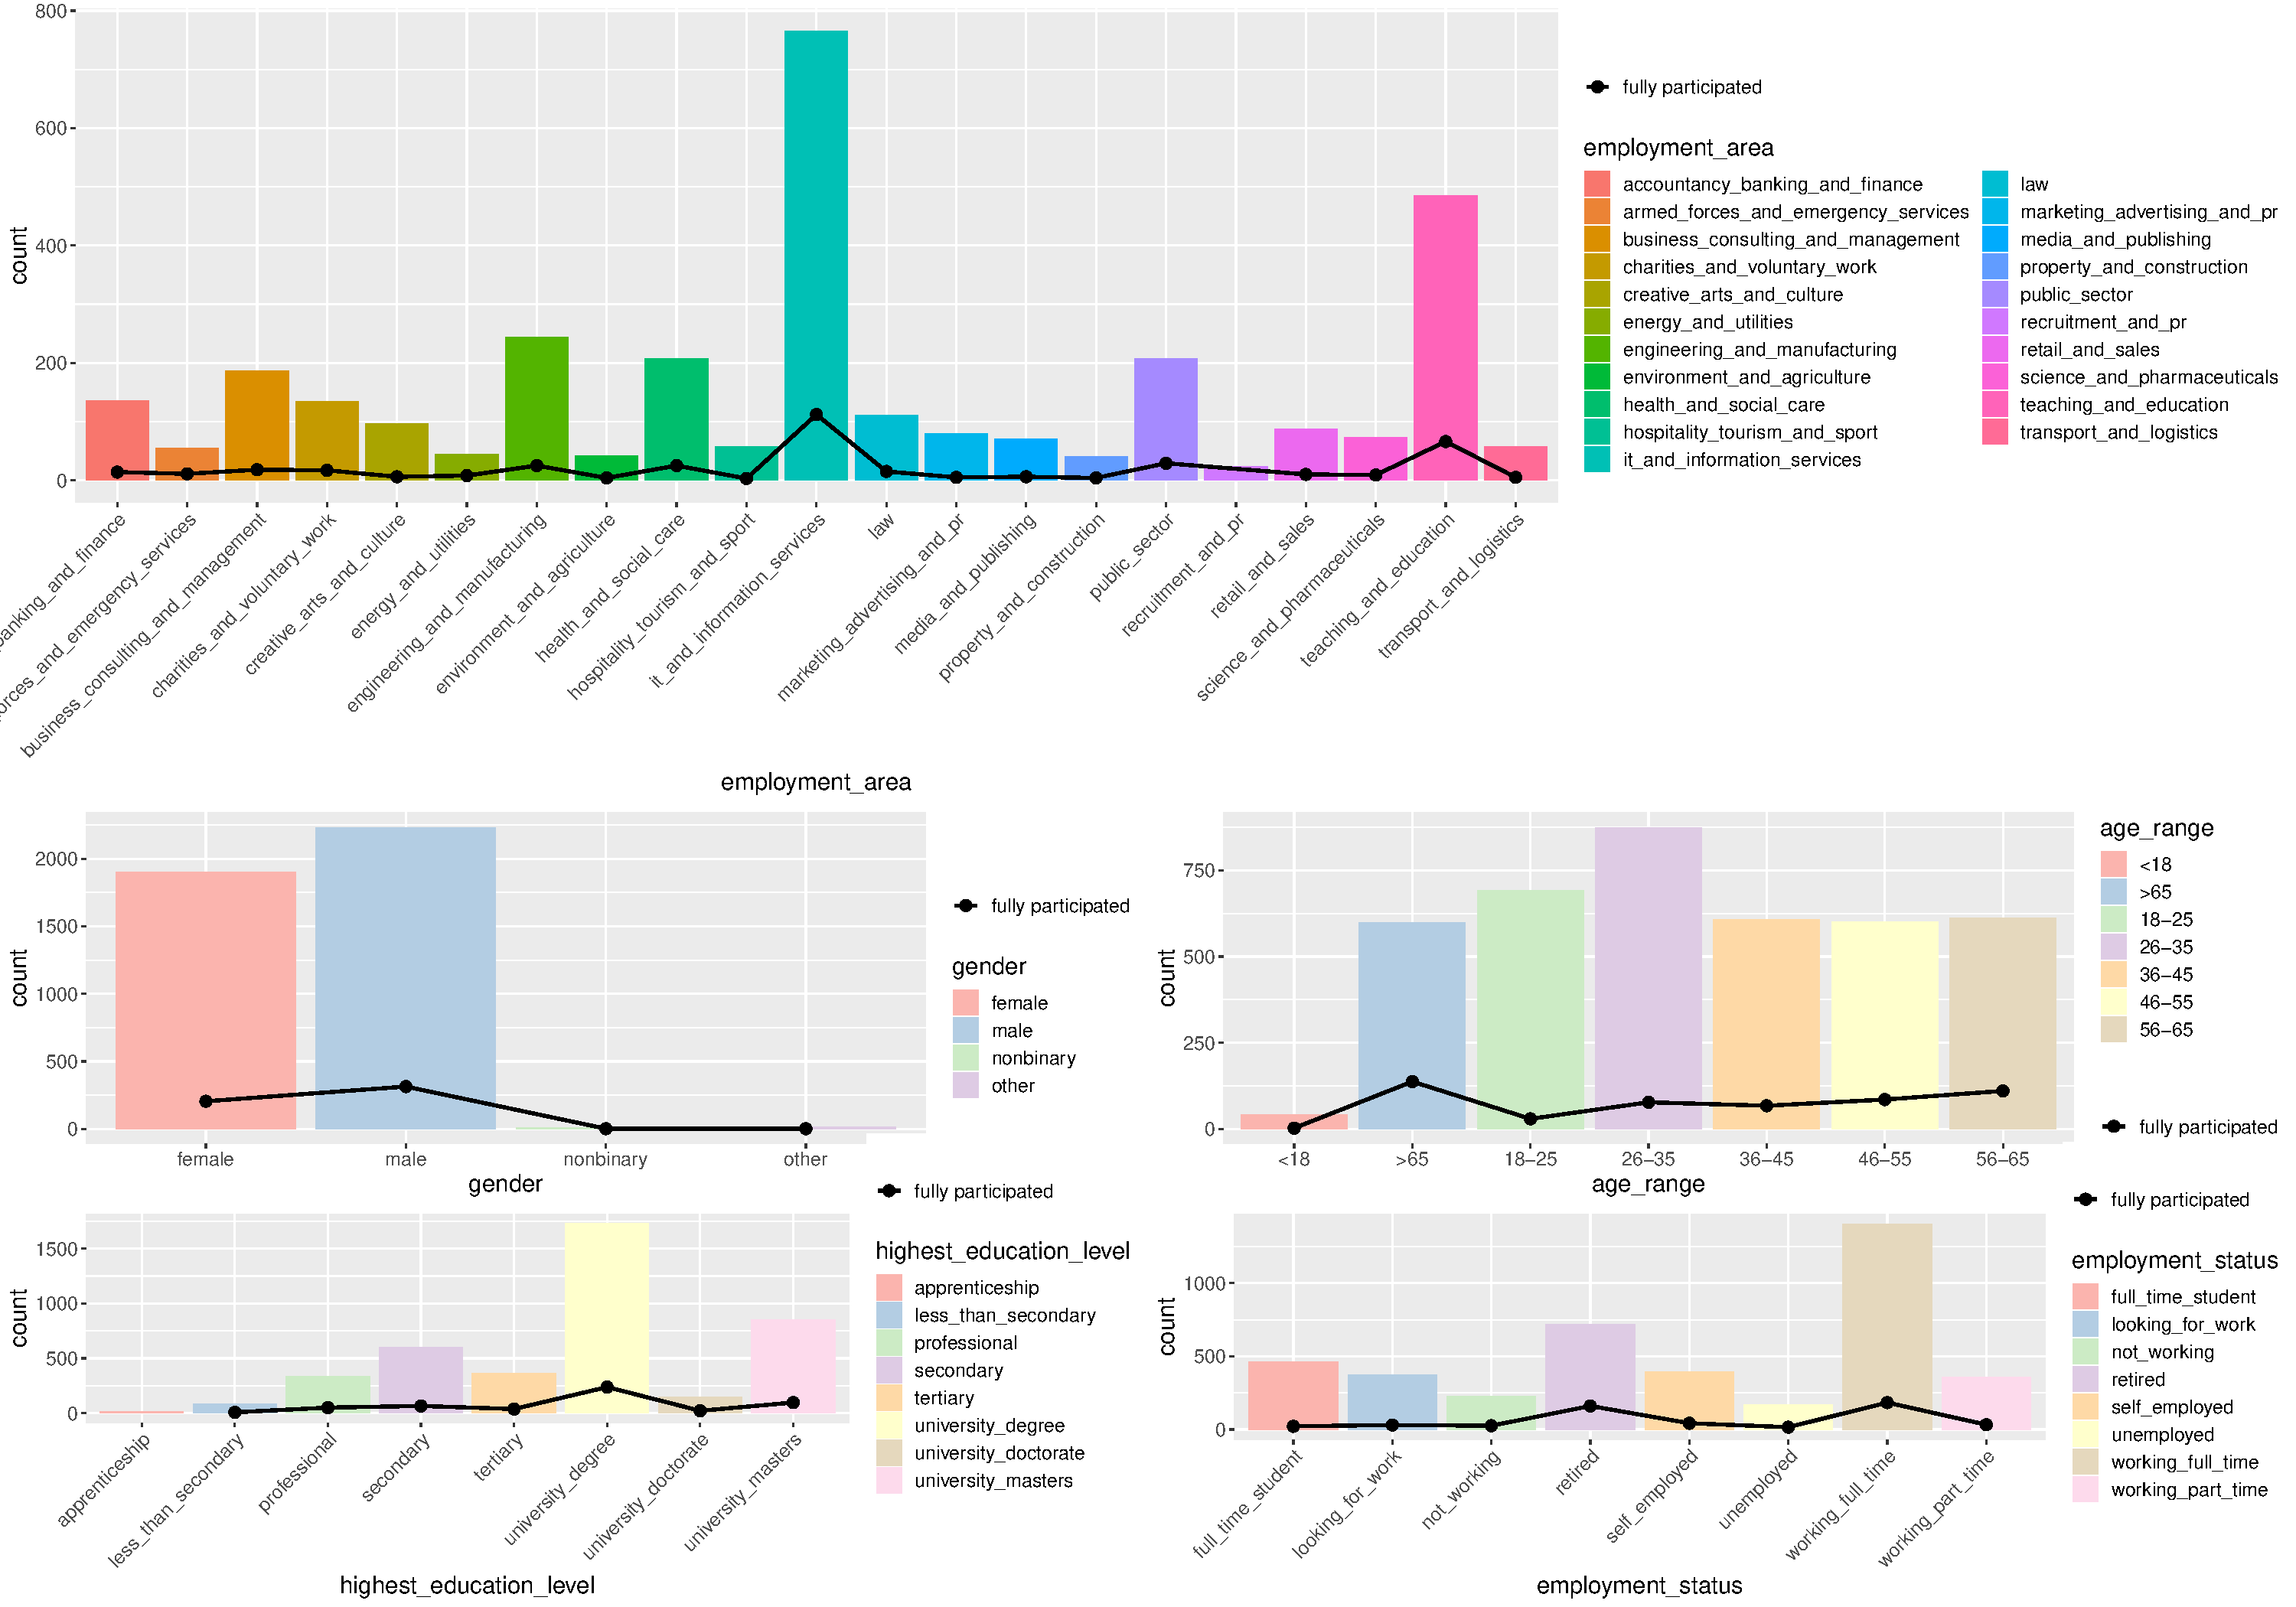
\includegraphics[width=1\linewidth]{CSC8631-Reports_files/figure-latex/unnamed-chunk-3-1} \caption{Enrolled and fully participated over different variables}\label{fig:unnamed-chunk-3}
\end{figure}

Now this graph, fig 3 shows the different characteristics of the
learners who enrolled and the learners who fully participated in the
course, i.e., they completed the course and purchased the course
certificate.

Here when we see the employment area of the learners, we see that people
from various domains have enrolled for the course but we can see that
most of the learners are from IT and Information Services background and
thus they are much interested in the course. The second dominating
employment area is Teaching and education. May be there is a possibility
that learners from these areas are pursuing this course for career
advancements in their field. The line graph represents the learners who
have fully participated (completed the course, i.e, that is purchased
the upgraded course certificates). Here we observe that they mostly
follow the same trend as enrolments in this case. We notice that from
the employment area, Recruitment and PR, none of the learners have
completed the course. This can be further checked and can be a future
scope of this project to see why this particular category doesn't have
any learner who completed the course.

The course offered, that is, Cyber Security (Cyber Security: Safety at
home, online, in Life) teaches about the cyber threats and the security
measures to be followed and is kind of related to the IT domain-based
course, so we can see that most of the learners are from that area and
thus are our target audience. Now, when we are aiming the other group of
learners, despite the course (as seen from the modules and the topics)
explains about the basic cyber safety rules that can be implemented in
daily lives, people from other backgrounds tend to be skeptical about
the course thinking that it might be on the very technical side and thus
not enrolling for the same. In this case we can focus on tailoring our
course in a way that it's understandable and approachable from learners
from varied backgrounds. One way can be introducing this course in two
levels as 1) Beginners and 2) Advanced. With this there is a possibility
that learners from different background will now be tempted and will
look forward to joining the Beginner level of the course to get familiar
with the topic and if they build a foundation, they will be interested
in enrolling for the next level of the course to get the knowledge of
the topic on whole. This can increase the reach and customer base for
our business. There will be a tradeoff with effort and timing but it can
be compensated with the profit made.

When we see the higher education level, we see that most of the learners
who enrolled, have completed their university degree. They are our
serious learners and our target audience. The approach that we used
previously to target learners from various other domains can be
beneficial here as well because then learners from any educational level
background will be comfortable in enrolling for the course. Here, we can
observe the learners who are on apprenticeship never fully participated
for the program.

Now when we are analyzing the age range, we can see that most of the
learners are from the age range 26-35. The second and third highest
number of learners are from the age range 18-25 and more than 65 years
respectively. Here we see that learners who are in the age range of more
than 65 years tend to fully participate in the course the most as
compared to others. Now, simultaneously if we see the employment status,
we can see the highest number of learners enrolled are working full time
and then the next highest number of learners are from the retired
category. Here again we observe that learners from retired category tend
to have fully participated in the course the highest as compared to
others. This analysis shows that learners who are retired (generally
they belong in the age range \textgreater65 years) tend to fully
participate in the course (i.e., compete the course and purchase the
upgraded certificate). It might be possible that they have some extra
free time as compared to those who are working or otherwise.

Another possible reason for the learners from the retired category and
the age group of more than 65 years of age to stay through the course
and fully participate in it, can have to do something with what the
course offers. Here we can see that the course is for cyber security
(safety at home, online, in Life), which is something that everyone
wants to have knowledge of. In a very general scenario, a very
significant number of people who are in the age group above 65 years or
so are not very well versed with technology and its applications and
they are trying to be in sync with the day-to-day applications of the
technology and internet in a safe and secure manner. In today's world
everything is connected via internet and everyone at some point of time
has to use it in daily life applications at some place. So, the senior
citizens who are starting to use the technology and the online smart
applications in their daily lives may be wanting to learn about the
privacy issues and keeping themselves safe from cyber fraud and crime.

Talking about the gender we can't say it is a very significant factor in
analysis as the number of male and female catch up to each other. We
even see that most of the learners belong to these two categories and
very few learners have mentioned their gender as others or non-binary.

\textbf{Analysing the Archetype of the learners to see how people intend
to use this course for }

For this analysis we are using our merged data from enrolment and
archetype dataset.Although we don't have archetype for batch 1 and batch
2, but here we are joining(left join) all the available data that we
have and then producing a broad overview of our analysis.

\begin{figure}
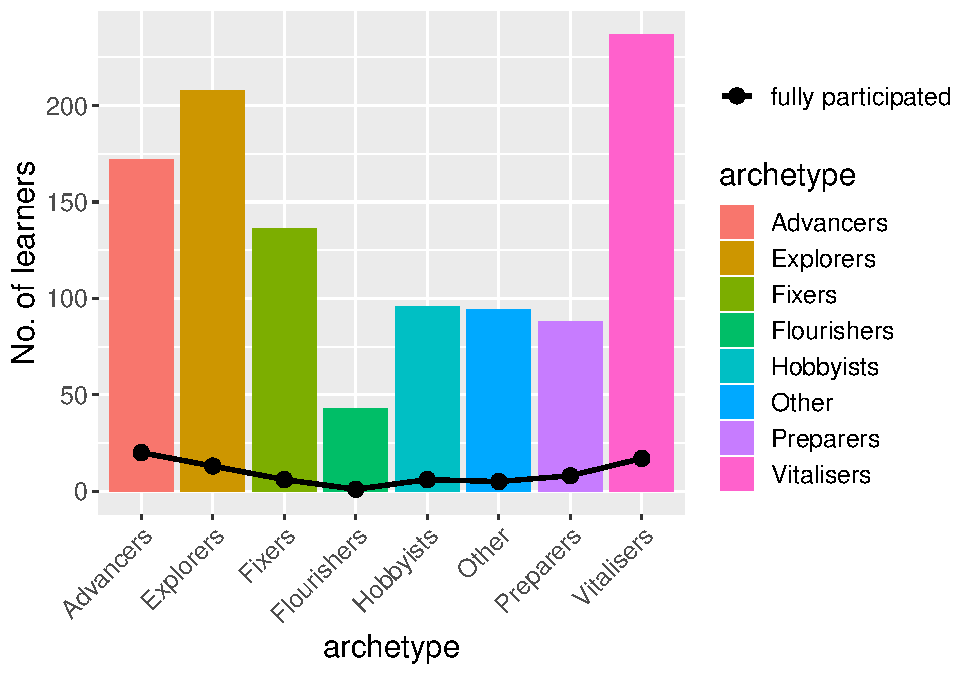
\includegraphics[width=1\linewidth]{CSC8631-Reports_files/figure-latex/unnamed-chunk-4-1} \caption{Archetype of the learners enrolled}\label{fig:unnamed-chunk-4}
\end{figure}

So now when we see the archetype of the learners, we see that the
highest number of learners who enrolled for the course are from the
category, vitalisers, explorers and advancers. Advancers rank 3rd in the
enrolment but their rate of full participation in the course is highest.
They are our most serious learners and they intend to use this course to
pick up additional work-related skills.

Explorers are considering a career change and are using this course to
evaluate their options. The number of enrolments for them is high too,
but they tend to full participate in the course less than the advancers.
Vitalisers enrolled the most but their rate of completion is less than
the advancers. They have joined this course as hobby just like
hobbyists.

Here it can be interpreted that learners from maybe IT background who
rank the most in employment area, want advancement in the same career
and thus tend fully participate in the course by purchasing the upgraded
course certification.

Overall if we see these data and their analysis, it tells us that
usually the learners who are from IT and Information services domain
tends to join the course more, again the people who are in the age range
of 26-35 and works full time and have completed the university degree
are our most enrolled learners but the rate of fully participation is
kind of on the lower side.

Moreover, earlier from fig 2 - the leaving response survey, we even saw
that learner who left the course and did not fully participate gave the
feedback of not having enough time and again we also analyzed that
mostly the learners belong to the employment status of working full time
and thus face difficulties in managing time for the course. Here one
solution to retain the learners from this category can be to expand the
duration of the course so that learners can spend a little less time
each week and thus end up completing the course at their convenience and
not leaving the course mid-way due to time crunch and thus we can reduce
the student drop out rate from our course.

We will now focus on analysing the weekly response or the feedback from
the learners to get an idea of how the learners have responded to our
course. For this we will be using the merged file from all the seven
batches of the weekly sentiment survey response data set.

The exploratory textual analysis of the weekly sentiment's dataset is
done by word cloud. It provides an excellent way to analyze the text
data through visualization and helps to find important words that can
help in extracting insights from the data through which we can
communicate the most salient points in the reporting. For this a vector
is created containing only the text and then the text data is loaded as
a corpus. Then the data was cleaned by removing the special characters,
numbers or punctuation from the text, as well as removing common stop
words and stripping the white spaces. Then a data frame is created
containing each word in the first column and their frequency in the
second column which was used to create our desired visualization.

\begin{figure}
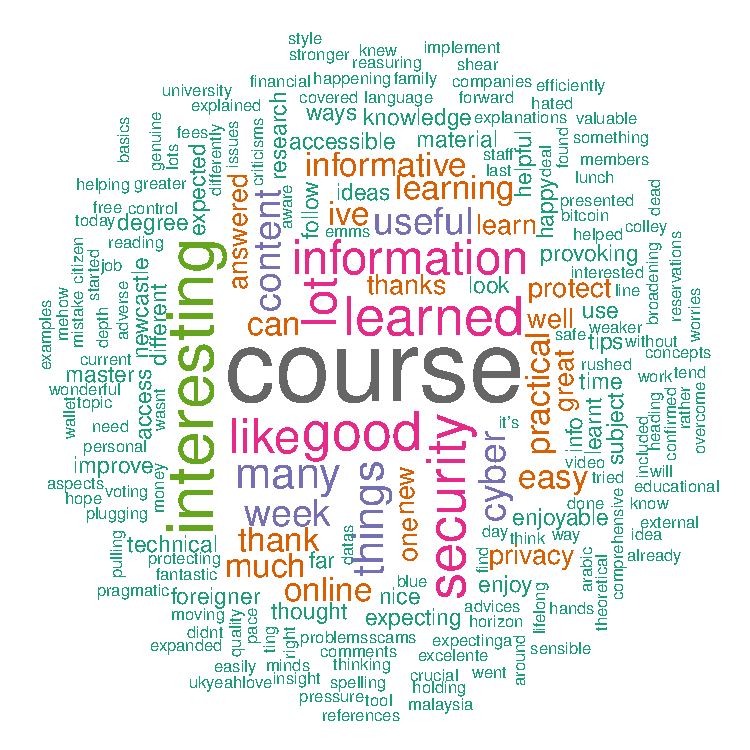
\includegraphics[width=1\linewidth]{CSC8631-Reports_files/figure-latex/unnamed-chunk-5-1} \caption{Weekly feedback about the course}\label{fig:unnamed-chunk-5}
\end{figure}

Now, when we see the weekly sentiment of the learners, in fig 5 , we
mostly have positive responses. So we can say that learners who fully
participated in the course , found the the contents positive and helpful
and are happy with the course. As analysed above we can infer that, as
we see most of the learners are from IT and Information services so
there is a possibility that they will feel familiar with the course and
are satisfied with the content. Here we can try streamlining our course
in a way that it would be helpful for learners from different
backgrounds and domains to increase our reach to diverse fields of
learners and adequately meet their requirements and expectations from
the course as well.

Now we can also target our audience from the countries, where the
learners enrolled the most.

We can analyse this on the basis of continents and further from the
countries.

For carrying out analysis for the continents for maximum number of
course videos watched by the learners, which in a way shows the maximum
participation from the continents, we used the merged video\_stats data
set from all the batches and calculated the column mean of view
percentage from every continent column. This data was then taken into
consideration.

\begin{figure}
\includegraphics[width=1\linewidth]{CSC8631-Reports_files/figure-latex/unnamed-chunk-6-1} \caption{Learners from all the continents}\label{fig:unnamed-chunk-6}
\end{figure}

Here we observe that view percentage from all the continents rank in the
order from highest to lowest starting with Europe, Asia, North America,
Africa,Oceania and South America. We see that we have no views from the
Antarctica. This is because we know that Antarctica is the only
continent with no permanent human habitation.

Now we will check the countries from where most of the learners enrolled
for the course from the all\_enrolments dataset (here as discussed
earlier we will consider the detected country column)

Here for this analysis the count of each country was stored in a column.
Now to compare the enrolments and the fully participated learners from
each country, the data was normalized because number of learners
enrolled were significantly more than the number of learners who fully
participated in the course. So to plot on similar axis, normalization
was needed.

\begin{figure}
\includegraphics[width=1\linewidth]{CSC8631-Reports_files/figure-latex/unnamed-chunk-7-1} \caption{Learners from the countries across the world}\label{fig:unnamed-chunk-7}
\end{figure}

Here we see that the enrolments from the top 10 countries follow the
trend of the learners enrolled from respective continents. This tells us
that our analysis is reliable. Here for example we see, Great Britain
has the highest number of enrolments followed by India and the US which
belongs to the top 3 continents ranked.

Here for concentrating on capturing more learners , we analyse which
part of the world attracts most of the learners and we will try to
strengthen the customer base in those areas more, plus try on tailoring
the course for the area from where the response is not satisfactory to
draw learners from those areas as well.

Fig 7 shows the enrolments from top 9 countries. We also observe that
the top 12 countries constitute the maximum number of learners and the
trend of fully participation in the course is kind of the same. So, we
will try aiming the learners from those countries so that we don't loose
our customer base.

Now, here we will evaluate the views and captions of the video content
for further analysis.

\begin{figure}
\includegraphics[width=1\linewidth]{CSC8631-Reports_files/figure-latex/unnamed-chunk-8-1} \caption{Analysis_of_total_views_HD_views_captions_Transcript_for_video_contents}\label{fig:unnamed-chunk-8}
\end{figure}

Fig 8 shows the trend of total views, how many people watched the video
with captions, who accessed the transcript and who watched the video in
HD mode.

We observe that the total views of the videos for every title differ a
lot. This shows that a lot of learners are interested in some particular
topic. Here we can see some video titles(steps) are viewed the more than
the others. One of the most watched video is the introductory video. The
second most watched video is `Privacy Online and Offline' -- Learners
are highly watching this video chapter because they might find it
important and interesting. Here from the agenda of the course and from
our analysis above, we have inferred that there is a possibility that
people are enrolling in this course to get an idea and understanding of
importance of cyber security in daily life. So, to avoid themselves from
being a victim of the cyber fraud they might have shown interest in this
topic.

The third most watched video is ``Why would anyone want your data'' -
The choice of most watched videos gives us an idea that learners want to
be aware of the data privacy issues and how they can safely use and
share their private data.

So, we can look for adding modules with similar content (detailed
content on the same kind of topic), which helps people with knowledge of
cyber security in day to day lives. This can help to draw attention of
the learners and will expand the customer base.

Now, if we see the trend of the HD viewing of the video content by the
learners, we can see that it shows a spike for a particular video
chapter. There can be few possibilities for this which needs to be
analyzed. There can be a chance that it might contain some important
pictorial information or graphs or something that needs to be evaluated
critically and so learners tend to watch it in HD. Or maybe there is a
chance that the video is not clear and thus learners turn on the HD view
to get a better visual. If that is the case, then immediate action
should be taken to handle this to maintain the quality of the course.

Again, we see that captions are provided for all the videos but very few
learners have turned on the captions. That can mean that the audio and
the contents of the lectures are projected to the audience very
effectively. This means that our analysis from the sentiment response
feedback holds true because there we saw that most of the comments are
positive for the course.

But the presence of captions and transcript makes the course very
versatile as it is particularly very beneficial from learners watching
the video in their non native language. This can attract the learners
from a very vast base.

\begin{center}\rule{0.5\linewidth}{0.5pt}\end{center}

Now again for any online course provider, one of the most important
criteria is to keep strengthening its online platform and making it more
user friendly.

\textbf{Business Objective }

\begin{itemize}
\tightlist
\item
  We want to focus on optimizing the user experience and learning
  environment and enhancing the learning experience
\end{itemize}

\textbf{Data Description }

Here for this analysis, we are using the merged video stats dataset from
all the seven batches to see what kind of devices people prefer most for
watching the course videos.

\textbf{Data Preparation: }

From the merged video stats dataset, the column mean for each device
column (desktop,mobile, tablet,tv and console) is calculated and taken
into consideration to get an idea of what kind of devices people are
using mostly for watching the content

\textbf{Evaluation/ Data Analysis:}

Now, online courses are highly dependent on how friendly the user
interface is for accessing the course and the materials. Here we will
analyse the types of devices use most for streaming the content.

Fig 8. gives the number of devices used for watching the video modules
of the course

\begin{figure}
\includegraphics[width=1\linewidth]{CSC8631-Reports_files/figure-latex/unnamed-chunk-9-1} \caption{Devices Used}\label{fig:unnamed-chunk-9}
\end{figure}

Here we see that most of the learners prefer watching the content on
desktop than on any other device. So the interface of the site must be
maintained for the desktop version and time to time upgradations should
be done. We can optimize the User Interface for the mobile and tablet
devices as well, so that learners can access the content easily at
anytime or anyplace (as mobiles and tablets are handy ) and thus there
are chances that we may see an increase in the rate of learners who can
fully participate. Because if they can access the course at ease of
their hand at any point of time then there is a possibility that they
will tend finish the course (as stated earlier learners complained that
they don't fully participate in the course and leave it midway as they
don't have enough time). So, if its handy, the learners might not feel
obligated to access the course from their study/work space, rather there
are chances that they will tend to watch at any point of time as it will
be accessible easily. This will upgrade and provide a better learning
platform.

Here we can see , almost no one use the console (very negligible amount)
or TV device to access the course. But keeping in mind that the data is
from 3 years ago, and now a days a lot of people use smart TV , so
keeping the future scope in mind, the company can focus on making the UI
of TV device user friendly too.

\hypertarget{conclusion}{%
\subsection{Conclusion :}\label{conclusion}}

We observe that most of the details about the learners enrolled are
unknown. There is a possibility that learners don't provide their
details because of some privacy issues or lack of knowledge about how
their data will be used. Here the course provider should put in place
the clear ethical policies and code of practices about how the student
data will be used in analytics. These policies should address student
privacy, security of data and the consent. From the evaluation and
analysis of datasets, we have inferred that most of the learners are
from IT and Information Services background and are in the age range of
26-35 years, but their rate of full participation(that is upgrading to
the purchase certification) is low. Comparatively, the learners in the
age range of 65 years or above, those who belong to the retired category
tend to fully participate in the course although their enrolment rate is
less.We also observed that most of the learners enrolled are from
Europe,Asia and North America, especially we can see a significant
number of learners from Great Britain, India and the US. So, we can say
that a huge influx of learners are from these categories.\\
Here we must focus on retaining our loyal customers(the learners) as
well as explore ways to attract learners from varied background and
categories. Simultaneously, we must work for the improvement and
enhancement of the course and figure out the shortcomings and work
proactively on them to maintain the quality of the program offered.

\end{document}
